\documentclass[12pt]{article}
\usepackage[utf8]{inputenc}
\usepackage{amsmath}
\usepackage{mathrsfs}
\usepackage{amssymb}
\usepackage{amsfonts}

\DeclareMathOperator{\logit}{logit}
\DeclareMathOperator*{\argmax}{arg\,max}
\DeclareMathOperator*{\argmin}{arg\,min}

\usepackage[
    a4paper,
    left = 2.5cm,
    right = 2.5cm,
    top = 2.5cm,
    bottom = 2.5cm
]{geometry}

\usepackage{graphicx}
\usepackage[headings]{fullpage}
\usepackage{hyperref}
\usepackage{fancyhdr}
\usepackage{units}
\usepackage{url}
 %For aligned formulas
 \usepackage{IEEEtrantools}
\usepackage{listings} %Source code listings https://en.wikibooks.org/wiki/LaTeX/Source_Code_Listings
\usepackage{xcolor}

\lstset{
    language=Python, %You can always set to another language
    breaklines=true,
    basicstyle=\ttfamily\footnotesize,
    keywordstyle=\color{blue}\bfseries,
    stringstyle=\color{orange},
    commentstyle=\color{gray}\itshape,
    showstringspaces=false,
    morekeywords={BasicWorkflow, CouplingFlow, TimeSeriesNetwork, SIR, fit_online, plot_default_diagnostics}, % your specific class names here
    tabsize=4
}

\usepackage[
    backend=biber,
    style=apa,
    maxcitenames=2,
    mincitenames=1,
    sorting=ynt
    ]{biblatex}
\addbibresource{bibfile.bib}

\setlength{\headheight}{15pt}
\pagestyle{fancy}
\fancyhf{}
\rhead{\footnotesize Kiana Ebrahimi Farbod, Samaneh Naghdbishi, Armin Maddah Asl, Geri Lila}
\lhead{SBI Project}
\rfoot{Page \thepage}


\begin{document}

\begin{titlepage}
        \centering % Center all text
        \vspace*{\baselineskip} % White space at the top of the page
        
        {\huge Inference of Protein Secondary Structure Motifs\\[0.1\baselineskip]
         with Hidden Markov Models and BayesFlow}\\[0.2\baselineskip]
        
        
        \vspace*{\baselineskip}
        
        {\Large --- Project Report ---\\
          Simulation Based Inference\\[\baselineskip]} % Tagline(s) or further description
        \vspace*{\baselineskip}
        

        {\LARGE 
            Kiana Ebrahimi Farbod, 284599\\[10pt]
            Student 2 name, matriculation number\\[10pt]
            Student 3 name, matriculation number\\[10pt]
            Student 4 name, matriculation number\\[10pt]
        } % Your names  
        
        \vfill

        \today \par % Location and year
        
        \vspace*{\baselineskip}

        {\itshape TU Dortmund University\par}
    \end{titlepage}

\clearpage

\section{Introduction}

Proteins are linear chains of amino acids that fold into complex three-dimensional structures
determining their biological function. An intermediate level of organization is the
\textit{secondary structure}, where each amino acid residue participates in local folding
patterns: $\alpha$-helices, $\beta$-sheets, or random coils \parencite{bioninja}.
Predicting secondary structure from sequence alone is a fundamental problem in computational
biology.

In this project, we formulate secondary structure prediction as a probabilistic inference
problem. We define a two-state Hidden Markov Model (HMM) with fixed transition and emission
probabilities derived from empirical protein data \parencite{kaggle}. The HMM's hidden states
represent $\alpha$-helix versus ``other'' (encompassing $\beta$-sheets and coils). Given an
amino acid sequence, the Forward-Backward algorithm \parencite{jurafsky} computes the exact
per-position posterior probability of each state — this serves as our ground truth.

We then train a neural posterior estimator using \textit{BayesFlow} \parencite{bayesflow}
to approximate these posteriors from amino acid sequences alone, without access to the HMM
parameters. We compare two training designs for the summary network that conditions
BayesFlow: a staged design that pretrains it separately and freezes it, and a joint,
end-to-end design that lets BayesFlow's own training signal shape it directly
(Section~\ref{sec:joint}). The trained models are validated on held-out simulated sequences
and on a real protein: human insulin (PDB: 1A7F) \parencite{insulin}.

The report is structured as follows: Section~2 describes the simulated data and insulin
validation set. Section~3 defines the HMM statistical model. Section~4 presents the neural
approximator architecture. Section~5 details the training pipeline. Section~6 covers
diagnostics and calibration. Section~7 reports inference results. Section~8 concludes.


\section{Data}

The data layer has two purposes. First, it produces an unlimited supply of simulated amino-acid sequences combined with exact per-residue inference targets. Second, it converts a real protein structure, human insulin 1A7F, into the same sequence representation and a compatible two-state validation target.

\subsection{Canonical representation}

Each amino acid is represented by an integer in {0, . . . , 19}. The canonical order used
throughout the project is
\begin{equation}
(\mathrm{A,R,N,D,C,E,Q,G,H,I,L,K,M,F,P,S,T,W,Y,V}).
\end{equation}
For example, alanine is encoded as 0, glycine as 7, and valine as 19. The mapping, inverse
mapping, state labels, and all probability arrays are defined once in
\texttt{encoding.py}. The hidden-state convention is $0=\alpha$-helix and
$1=\text{other}$. Probability vectors and matrix rows are checked at import time to
ensure that they sum to one.

The common representation is important since the simulator generates integer sequences, which are similar to those used by the \texttt{hmmlearn} algorithm. As a result, the pre-processing stage of the insulin molecule has to produce an input sequence compatible with the representation generated through simulation. It is important to note that the full alphabet size is always equal to 20, even for short sequences without the last symbol.

\subsection{Simulated training data}

The training examples are generated directly using the two-state fixed Hidden Markov Model (HMM) mentioned in Section 3. For the requested length $L$, the simulator will generate two sequences in alignment: the sequence of states $s_{1:L}$ and the sequence of amino acids $x_{1:L}$. The sequence of states will be generated in sequence to account for the Markov dependence. With this sequence, emissions in positions that are associated with the same state will be generated together, avoiding an extra amino acid generation step for each position.

All randomness is supplied through a NumPy \texttt{Generator}. Consequently, a fixed
seed reproduces sequence lengths, state paths, and emitted amino acids exactly. For a
batch of $n$ examples, lengths are sampled independently from the discrete uniform
distribution
\begin{equation}
L_i \sim \mathcal{U}\{10,11,\ldots,60\}, \qquad i=1,\ldots,n.
\end{equation}
This range covers both short insulin chains while retaining longer sequences that show
several state transitions. Dataset size is not intrinsic to the simulator: the training
script can request as many examples as required. In the final training configuration,
2000 training sequences and 400 validation sequences were generated, with independent
held-out sequences generated for evaluation.

The simulator retains the sampled state path even though the neural target is the
Forward-Backward posterior. The state path is useful for diagnostics of the generative
process and for any later comparison between posterior probabilities and the latent state
that generated a sequence.

\subsection{Exact targets and dataset handoff}

For every simulated observation $x_{1:L}$, exact HMM inference produces
\begin{equation}
y_t = P(S_t=0\mid X_{1:L}=x_{1:L}), \qquad t=1,\ldots,L,
\end{equation}
where state 0 denotes $\alpha$-helix. Thus one training item consists of the integer
sequence, its per-position $\alpha$ posterior, and the sampled state path. The target is
a probability in $[0,1]$, not a hard classification label.

Since sequences have variable length, storing every example in a single padded matrix would introduce unnecessary padding. Instead, sequences are concatenated into a one-dimensional array and accompanied by a vector of sequence lengths.

A saved .npz file contains sequences
(integer observations), posteriors (floating-point targets), states (integer latent paths),
and lengths. Cumulative sums of lengths allows exact reconstruction of the example sequence. The model doesn’t need object arrays and pickling; it is portable and allows the system to know how to pad and mask itself. Table~\ref{tab:data-interfaces} shows the main interfaces that are exposed to the rest of the system.

\begin{table}[ht]
    \centering
    \caption{Data-layer modules and their interfaces.}
    \label{tab:data-interfaces}
    \footnotesize
    \begin{tabular}{p{0.25\textwidth}|p{0.65\textwidth}}
        \hline
        Module & Responsibility \\
        \hline
        \texttt{encoding.py} & Canonical amino-acid indices, state convention, and fixed HMM probability arrays. \\
        \texttt{simulator.py} & Seeded sampling of individual or batched state paths and amino-acid sequences. \\
        \texttt{forward\_backward.py} & Exact posterior targets, dataset generation, and lossless \texttt{.npz} save/load routines. \\
        \texttt{insulin.py} & Parsing and encoding of 1A7F chains and construction of experimental binary helix labels. \\
        \texttt{sanity\_check.py} & Monte Carlo validation of start, transition, and emission frequencies. \\
        {\raggedright\texttt{check\_forward\_\allowbreak backward.py}\par} & Independent correctness, probability, reproducibility, and round-trip checks. \\
        \hline
    \end{tabular}
\end{table}

\subsection{Insulin 1A7F validation data}

Human insulin 1A7F is used as an out-of-simulation validation example
\parencite{insulin}. The structure is an NMR entry containing two peptide chains. Chain A
has 21 residues and matches the wild-type human insulin A-chain sequence:
\begin{center}
\small\texttt{GIVEQCCTSICSLYQLENYCN}.
\end{center}
Chain B is the 29-residue mutant sequence
\begin{center}
\small\texttt{FVNQHLCGSHLVEALELVCGERGGFYTPK}.
\end{center}
Relative to the wild-type B chain, it contains the substitutions B16
Tyr$\rightarrow$Glu and B24 Phe$\rightarrow$Gly and lacks residue B30 (des-B30).

The mmCIF file was downloaded from the RCSB Protein Data Bank and then parsed using Biopython. All amino-acid residues that appeared in the first NMR model and adhered to the standard residues were selected. The three-letter codes for these residues were transformed into their respective one-letter codes and then into integers, as used by the simulator. The secondary structure annotation information was obtained from the {\_struct\_conf} records in the deposited PDB file. It is worth noting that only the residues belonging to class 1 helices (right-handed $\alpha$-helices) were classified as positive while others as “other.” The annotated ranges and
class balance are shown in Table~\ref{tab:insulin-data}.

\begin{table}[ht]
    \centering
    \caption{Processed 1A7F validation chains. Helix ranges use deposited author residue numbering.}
    \label{tab:insulin-data}
    \begin{tabular}{c|c|c|c|c}
        \hline
        Chain & Length & $\alpha$-helix ranges & $\alpha$ residues & $\alpha$ fraction \\
        \hline
        A & 21 & A2--A7, A13--A19 & 13 & 61.9\% \\
        B & 29 & B9--B18 & 10 & 34.5\% \\
        \hline
    \end{tabular}
\end{table}

These experimental labels are hard values: 1 denotes an annotated $\alpha$-helical
residue and 0 denotes other. They are not Forward-Backward posteriors and are never used
to train the model. For file-format compatibility, they occupy the dataset's
\texttt{posteriors} field, while the corresponding HMM-style state array uses the project
convention $0=\alpha$ and $1=\text{other}$. The preprocessing verifies the expected sequences and chain lengths, confirms that the helix annotations and binary labels align with the corresponding residues, and reloads the saved dataset to ensure that no information changes during storage.

\section{Statistical model}

\subsection{Two-state Hidden Markov Model}

Define $S_t\in\{0,1\}$ to be the state of the secondary structure at position $t$, where $S_t=0$ represents an $\alpha$-helix and $S_t=1$ represents “other”. The other state includes the $\beta$-sheet and random coil secondary structures. Let $X_t\in\{0,\ldots,19\}$ represent the amino acid at that position. The assumptions underlying the model are that the process is a first-order Markov process and that observations are conditionally independent given the current state:

\begin{equation}
P(s_{1:L},x_{1:L})
= P(s_1)P(x_1\mid s_1)
  \prod_{t=2}^{L} P(s_t\mid s_{t-1})P(x_t\mid s_t).
\label{eq:hmm-joint}
\end{equation}

The initial distribution is deterministic:
\begin{equation}
\boldsymbol{\pi}
=\begin{bmatrix}P(S_1=0)&P(S_1=1)\end{bmatrix}
=\begin{bmatrix}0&1\end{bmatrix}.
\label{eq:start}
\end{equation}
Every simulated sequence therefore starts in the other state. State transitions follow
the row-stochastic matrix
\begin{equation}
\mathbf{A}=
\begin{bmatrix}
P(0\mid0)&P(1\mid0)\\
P(0\mid1)&P(1\mid1)
\end{bmatrix}
=
\begin{bmatrix}
0.90&0.10\\
0.05&0.95
\end{bmatrix}.
\label{eq:transition}
\end{equation}
Thus an $\alpha$-helix continues with probability 0.90, while an other segment continues
with probability 0.95. The expected run lengths are $1/(1-0.90)=10$ residues for the
$\alpha$ state and $1/(1-0.95)=20$ residues for the other state. Solving
$\boldsymbol{\mu}=\boldsymbol{\mu}\mathbf{A}$ gives the stationary distribution
$\boldsymbol{\mu}=(1/3,2/3)$. The deterministic start distribution differs from this
stationary distribution, so short sequences are initially more strongly biased toward
the other state.

The state-conditional emission probabilities are fixed to the empirical values in
Table~\ref{tab:emissions}. Each row is a categorical distribution over the canonical
amino-acid order and sums to one.

\begin{table}[ht]
    \centering
    \caption{Emission probabilities (\%) for the two HMM states.}
    \label{tab:emissions}
    \footnotesize
    \setlength{\tabcolsep}{2.4pt}
    \begin{tabular}{l|rrrrrrrrrrrrrrrrrrrr}
        \hline
        State & A & R & N & D & C & E & Q & G & H & I & L & K & M & F & P & S & T & W & Y & V \\
        \hline
        $\alpha$ & 12 & 6 & 3 & 5 & 1 & 9 & 5 & 4 & 2 & 7 & 12 & 6 & 3 & 4 & 2 & 5 & 4 & 1 & 3 & 6 \\
        other & 6 & 5 & 5 & 6 & 2 & 5 & 3 & 9 & 3 & 5 & 8 & 6 & 2 & 4 & 6 & 7 & 6 & 1 & 4 & 7 \\
        \hline
    \end{tabular}
\end{table}

The emission table is intentionally simple. For example, alanine and leucine are more
probable under the $\alpha$ state, while glycine and proline are more probable under the
other state. However, the distributions overlap substantially; individual residues are
not decisive, and inference must combine evidence across the full sequence with the
persistence encoded in $\mathbf{A}$.

\subsection{Generative process}

Sequence of length $L$ was generated through the following steps:
\begin{enumerate}
    \item Set $S_1=1$ according to the initial distribution in
    Equation~\ref{eq:start}.
    \item For $t=2,\ldots,L$, draw $S_t\sim\operatorname{Categorical}
    (\mathbf{A}_{S_{t-1},:})$.
    \item At every position, draw $X_t\sim\operatorname{Categorical}
    (\mathbf{B}_{S_t,:})$, where $\mathbf{B}$ is the emission matrix in
    Table~\ref{tab:emissions} divided by 100.
\end{enumerate}
The process produces both the observation $x_{1:L}$ and its latent path $s_{1:L}$.
The neural approximator does not receive the path. Instead, it is trained on the exact
posterior marginals computed from the observation alone.

\subsection{Forward-Backward inference}

Because all HMM parameters are known, the posterior probability of each state can be
computed exactly with the Forward-Backward algorithm \parencite{jurafsky}. Define the
forward quantity
\begin{equation}
f_t(j)=P(X_{1:t}=x_{1:t},S_t=j)
\end{equation}
and the backward quantity
\begin{equation}
b_t(i)=P(X_{t+1:L}=x_{t+1:L}\mid S_t=i).
\end{equation}
With emission probability $B_{j,x_t}=P(X_t=x_t\mid S_t=j)$, their recursions are
\begin{align}
f_1(j) &= \pi_j B_{j,x_1}, \\
f_t(j) &= B_{j,x_t}\sum_{i=0}^{1} f_{t-1}(i)A_{ij},
          &&t=2,\ldots,L, \\
b_L(i) &= 1, \\
b_t(i) &= \sum_{j=0}^{1}A_{ij}B_{j,x_{t+1}}b_{t+1}(j),
          &&t=L-1,\ldots,1.
\end{align}
The smoothed posterior marginal is then
\begin{equation}
\gamma_t(j)
=P(S_t=j\mid x_{1:L})
=\frac{f_t(j)b_t(j)}{\sum_{k=0}^{1}f_t(k)b_t(k)}.
\label{eq:gamma}
\end{equation}
The training target is the $\alpha$ column, $y_t=\gamma_t(0)$.

This implementation uses \texttt{hmmlearn.CategoricalHMM} directly \parencite{hmmlearn}. The arrays \texttt{startprob\_}, \texttt{transmat\_}, and \texttt{emissionprob\_} are taken from the common constants, while the alphabet size is fixed at 20. No fitting is done: invoking \texttt{.fit()} function would change the parameters and no longer would correspond to the intended HMM. In a batch, variable length sequences are concatenated into a column vector and given along with their respective lengths. \texttt{predict\_proba} performs the inference independently for each sequence and provides both posterior columns, keeping column 0 as a target.

\subsection{Independent correctness check}

A two-residue observation provides a transparent check of the transition orientation and
emission indexing. Consider $x=(\mathrm{G},\mathrm{A})$, corresponding to indices $(7,0)$.
Since every sequence starts in the other state,
\begin{equation}
f_1=\begin{bmatrix}0&0.09\end{bmatrix}.
\end{equation}
At the second position,
\begin{align}
f_2(0)&=0.09\times0.05\times0.12=0.00054,\\
f_2(1)&=0.09\times0.95\times0.06=0.00513.
\end{align}
Therefore
\begin{equation}
P(S_2=0\mid \mathrm{G,A})
=\frac{0.00054}{0.00054+0.00513}
=0.095238\ldots,
\end{equation}
while $P(S_1=0\mid\mathrm{G,A})=0$ because of the deterministic start. The library
output matches this result and an independent NumPy implementation. Six additional
length-two and length-three sequences also match the independent recursion.

\subsection{Verification and reproducibility}

The simulator was evaluated involving 2000 independently generated sequences, 500 elements long, with seed 12345. The maximum difference between empirical and specified transition probabilities reached 0.0004, and that of the emission-probabilities is 0.0007, both of which are far lower than the defined Monte Carlo threshold of 0.01.

The Forward-Backward algorithm verification involved generating 200 sequences to ensure that the posterior values are within the range of [0,1], the two state probabilities' total at each location is equal to 1, and posterior value of alpha position 0 is precisely 0 for each sequence. Generation of the data sets using the same seed yielded identical results, observations, posterior values, and latent sequences. Moreover, saving and loading operations recreated exactly all array data. The present automated test suite in Section 2--3 involves 45 tests that all pass.

\subsection{Interpretation and limitations}

Given a fixed set of HMM parameters, (\ref{eq:gamma}) becomes a deterministic function of the sequence. Therefore, the neural network downstream has to approximate the exact computation of the Forward Backward algorithm instead of trying to learn an HMM parameter from a distributional prior. It is perhaps better thought of as amortized distillation of a supervised method for exact probability computations. It also goes on to explain the need for simulation-based calibration in following parts since the targets are sequence-specific marginal posteriors.

The HMM is intentionally constrained to be simple. The $\beta$-sheets and random coils are collapsed into one state, emission probabilities are not position-dependent, and the transition and emission probabilities are set to be constant values. The starting state being the deterministic other state ensures that the exact zero probability for $\alpha$ exists at the beginning of each sequence. Lastly, the target labels used in insulin sequences were generated through the experimental structures annotation and hence represent hard-labels, while simulated targets represent soft-HMM posteriors.

\section{Approximator}
\label{sec:approx}

\subsection{Architecture overview}

We use BayesFlow \parencite{bayesflow} to train a neural posterior estimator. The
architecture consists of two components:

\begin{enumerate}
    \item \textbf{Summary network:} A bidirectional LSTM (BiLSTM) that processes the
    variable-length amino acid sequence and produces a fixed-size summary vector.
    We use a BiLSTM rather than a permutation-invariant network because amino acid
    sequences have a meaningful sequential order — the position of each residue
    matters for secondary structure prediction.
    \item \textbf{Inference network:} A \texttt{CouplingFlow} normalizing flow
    \parencite{couplingflow} that learns the conditional density of the per-position
    $\alpha$-helix posteriors given the sequence summary.
\end{enumerate}

The BiLSTM architecture is: $\text{Embedding}(21) \to \text{BiLSTM}(\text{dim}=64)
\to \text{masked mean pooling} \to \text{Linear+ReLU} \to \text{summary}(\text{dim}=64)$.
A separate linear \texttt{position\_head} produces per-position logits for direct
point prediction of $P(\alpha)$. Padding token 20 is used for variable-length
sequences; \texttt{pack\_padded\_sequence} ensures the LSTM does not waste computation
on padded positions. The masked binary cross-entropy loss averages only over real
(non-padded) positions.

\subsection{Two-stage design}

Training proceeds in two stages, reflecting the fact that the summary network is not
differentiated through BayesFlow's flow loss:

\begin{enumerate}
    \item \textbf{Stage 1 — BiLSTM pretraining:} The summary network is trained
    directly on the masked BCE objective against Forward-Backward $\alpha$-helix
    posteriors, with an auxiliary loss predicting each sequence's mean $\alpha$-helix
    fraction. This ensures both the \texttt{position\_head} and \texttt{summary\_head}
    are well-trained.
    \item \textbf{Stage 2 — CouplingFlow training:} The BiLSTM is frozen. For each
    sequence, we compute a fixed-size condition vector by concatenating the pooled
    summary (dim~64) with the per-position logits (padded to \texttt{max\_len}=60,
    dim~60). The CouplingFlow (hidden widths~128, affine transform, actnorm; depth
    chosen by the search described in Section~\ref{sec:training})
    is then trained via \texttt{BasicWorkflow.fit\_offline} on
    $\{\text{condition} \to P(\alpha \mid \text{sequence})\}$.
\end{enumerate}

Raw logits (not sigmoid probabilities) are used in the condition because the
CouplingFlow's base distribution is an unconstrained Gaussian, and a second $[0,1]$-bounded
signal would destabilize training.

\subsection{Joint (end-to-end) alternative}
\label{sec:joint}

We also trained the alternative the two-stage design avoids: letting gradients
from the CouplingFlow's loss reach the BiLSTM directly, with no freezing step.
This works because BayesFlow runs on Keras 3's \texttt{torch} backend, where a
Keras layer is a \texttt{torch.nn.Module}; wrapping the same BiLSTM in
\texttt{keras.layers.TorchModuleWrapper} lets \texttt{BasicWorkflow} call it as
a real summary network every step, instead of consuming a precomputed
condition. Everything else is identical - dataset, BiLSTM architecture,
CouplingFlow, model-selection criterion (Section~\ref{sec:training}) - and
results are reported alongside the frozen design throughout
Sections~\ref{sec:training}--\ref{sec:inference}.


\section{Training and Diagnostics}
\label{sec:training}

\paragraph{Two-stage design and data regime.}
Training is offline: a fixed set of 2000 training and 400
validation sequences (length $10$--$60$, padded to $60$) is generated once
and reused across every epoch. The pipeline runs in two stages: first the
summary network (Section~\ref{sec:approx}) is pretrained to approximate the
Forward--Backward posteriors position by position and once that is done it
is frozen and reused purely as a feature extractor to condition the
coupling flow. Splitting the problem this way keeps each optimisation
target well defined: the summary network has a direct supervised signal to
fit and by the time the flow trains, that signal is no longer shifting
underneath it. All losses and metrics are computed on real positions only;
padding is excluded throughout.

\paragraph{Stage 1: summary-network pretraining.}
The network minimises a masked binary cross-entropy against the soft
Forward--Backward targets, using AdamW (learning rate $10^{-3}$, weight
decay $10^{-4}$), batch size $64$, gradient clipping at norm $1.0$ and a
\texttt{ReduceLROnPlateau} schedule, training for up to $60$ epochs with
early stopping (patience $8$). Its output forms a $124$-dimensional
condition: a $64$-dimensional pooled summary concatenated with the $60$
per-position logits. Both halves turn out to matter: an earlier version
conditioned the flow on the pooled summary alone, which discarded
positional information and performed worse than a sequence-blind baseline;
concatenating the per-position logits back in fixed that.

\paragraph{Stage 2: coupling-flow training and model selection.}
With the summary network frozen, the flow is trained with AdamW (learning
rate $5\times10^{-4}$, weight decay $10^{-3}$), batch size $64$, for $100$
epochs. One subtlety worth flagging: the flow's objective is a negative
log-density, so it is negative-valued and unbounded below. Roughly $44\%$
of every padded target is exactly zero (padding, plus the deterministic
state at position~$0$) and a continuous flow can place arbitrarily high
density on a single point, pushing the loss toward $-\infty$. Picking the
best configuration by this loss would just reward whichever one overfits
the padding hardest, so instead we rank configurations by masked mean
absolute error (MAE) against the Forward--Backward posteriors on real
positions. A search over optimiser, learning rate, depth, and weight decay
(six configurations) selected a coupling-flow depth of $10$
(Figure~\ref{fig:training}).

\paragraph{Convergence.}
The Stage-1 loss plateaus around $0.46$ (Figure~\ref{fig:training})
instead of going to zero, which looks like stalling but it isn't. For soft
probability targets, cross-entropy is bounded below by the mean entropy of
those targets rather than by zero. On the validation set that entropy
floor works out to $0.4621$ and the trained network reaches $0.4623$, a
gap of only $0.0003$. The flat curve is the loss sitting right at its
theoretical minimum. Training and validation losses track each other
closely throughout, so there is no sign of overfitting.

\paragraph{Calibration and coverage.}
Because the Forward--Backward posterior is a deterministic function of the
sequence, there is no classical parameter uncertainty here. What the
flow's spread reflects instead is uncertainty coming from the lossy
summary condition and the checks below assess that amortised uncertainty
specifically. On a separate held-out set of 200 test sequences (6764 real
positions), the rank histogram comes out close to uniform (mean rank
$0.528$, Kolmogorov--Smirnov distance $0.110$). After trimming the small
fraction of extreme-outlier draws ($|z|<4$; $63$ of $6564$ real-valued
z-scores clipped), $z$-scores have mean $0.13$ and standard deviation
$0.71$, and the nominal $90\%$ credible intervals achieve $96.1\%$
empirical coverage. A little conservative, which is the safer direction to
be wrong in. Most of the remaining deviation traces back to a boundary
effect. The deterministic and padded exact-zero positions cannot be
represented as point masses by a continuous flow, however well it is
trained.

\begin{figure}[t]
\centering
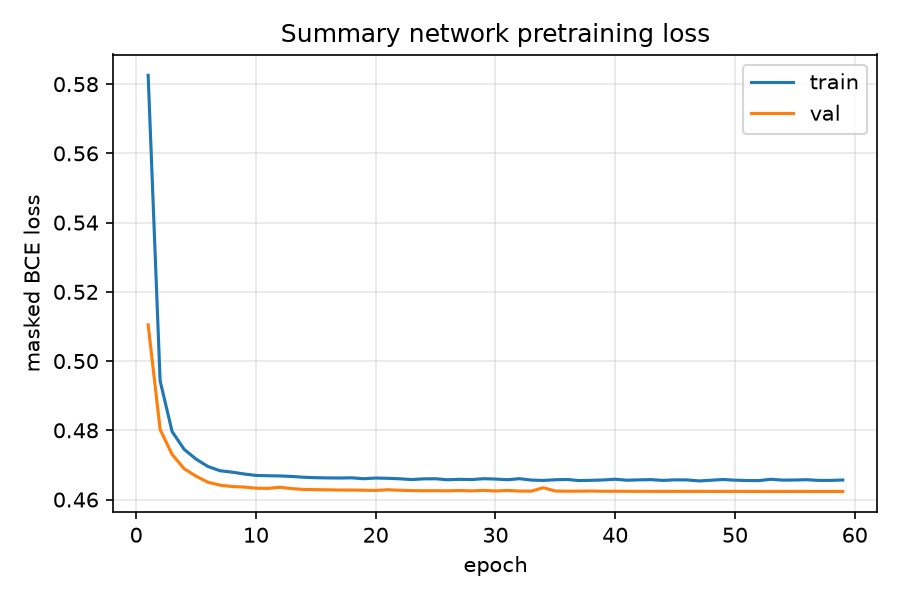
\includegraphics[width=0.48\linewidth]{figures/pretrain_loss.png}\hfill
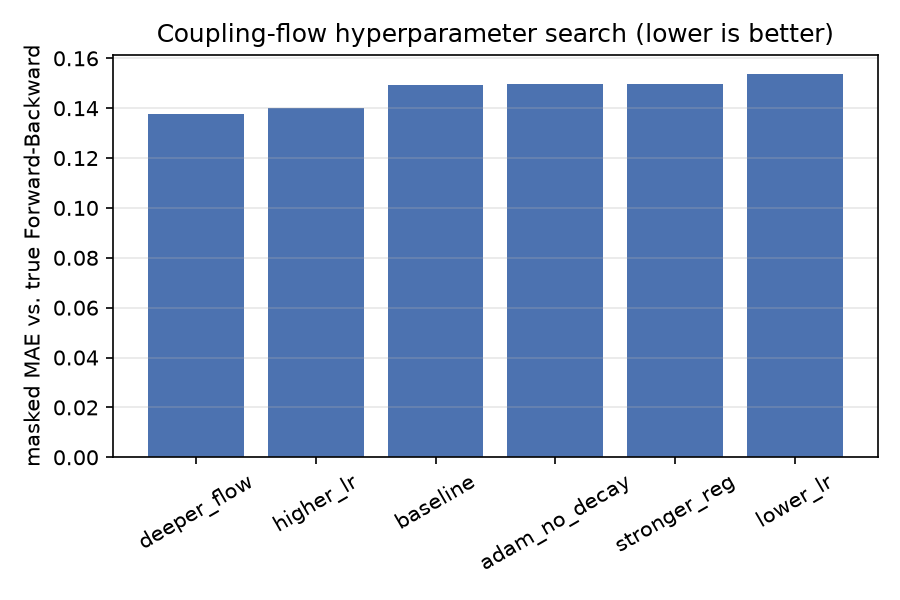
\includegraphics[width=0.48\linewidth]{figures/hyperparameter_search.png}
\caption{Left: Stage-1 pretraining loss; the plateau at $\approx 0.462$
coincides with the entropy floor of $0.4621$, indicating
convergence. Right: masked MAE per configuration (lower is better); the
depth-$10$ configuration was selected.}
\label{fig:training}
\end{figure}

\paragraph{Joint training: configuration and cost.}
The joint model reuses the same BiLSTM and CouplingFlow architectures, but
\texttt{fit\_offline} manages a single optimizer for the whole model (one
AdamW-with-cosine-warmup schedule), not the staged design's two
independently-tuned ones. The hyperparameter search was trimmed to four
configurations, since joint training pays the BiLSTM's forward/backward
cost on every step of every trial rather than once (Stage~1 amortises it
for the staged search). The search selected learning rate $10^{-3}$,
weight decay $10^{-3}$, depth~$6$. On this (CPU-only) machine the final
$100$-epoch retrain took $33.5$ minutes, versus $\sim17$ minutes for the
whole $4$-configuration search.

\begin{figure}[t]
\centering
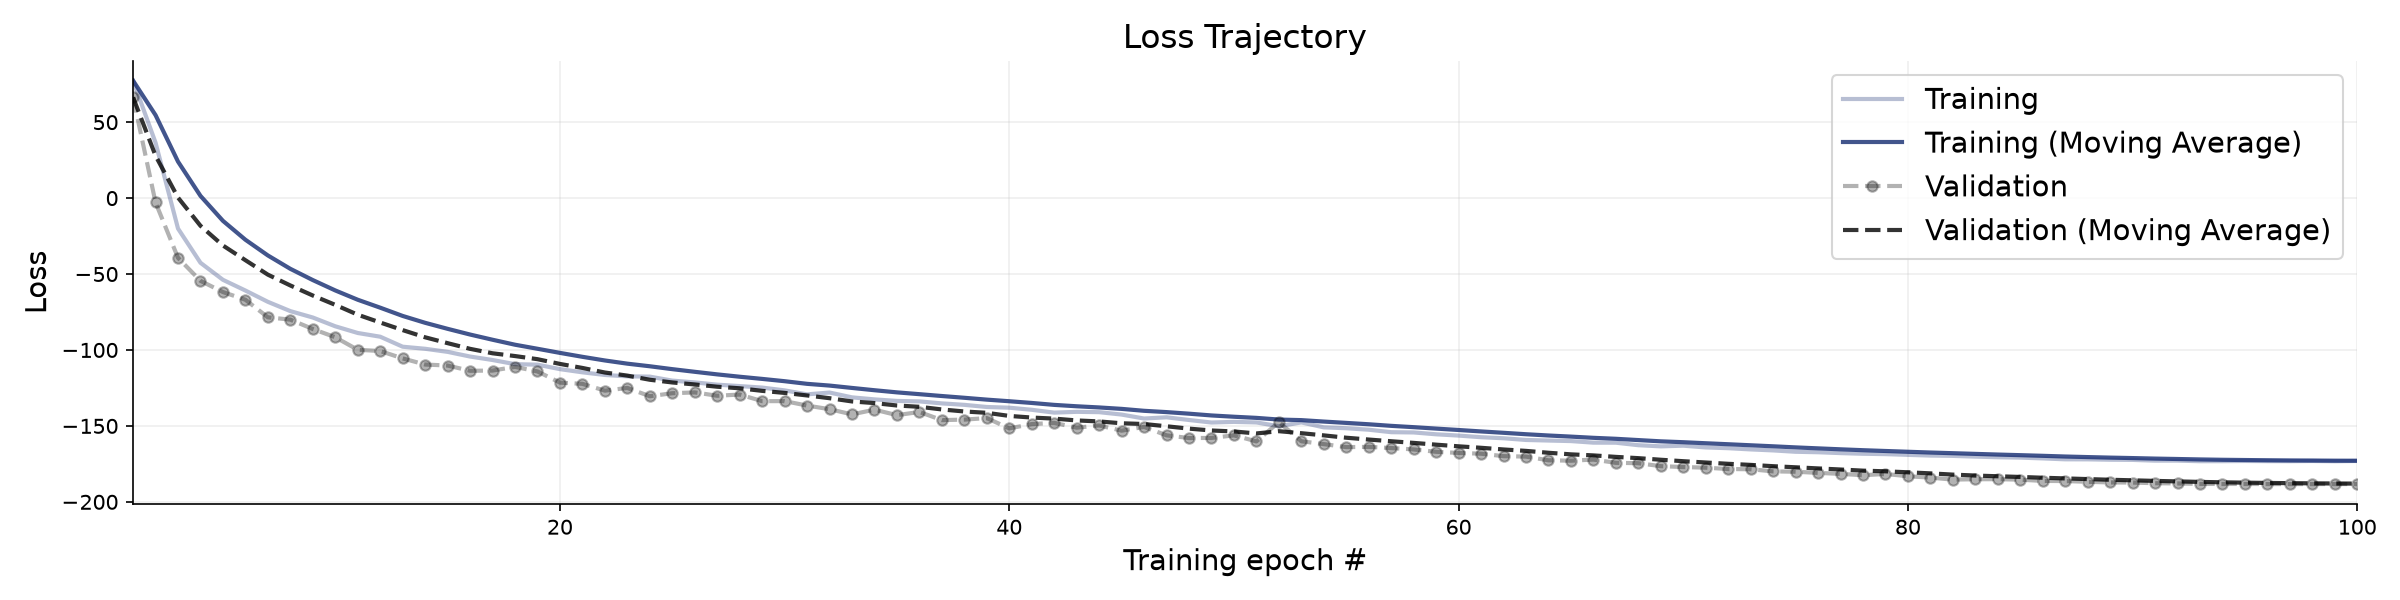
\includegraphics[width=0.48\linewidth]{figures/joint_loss.png}\hfill
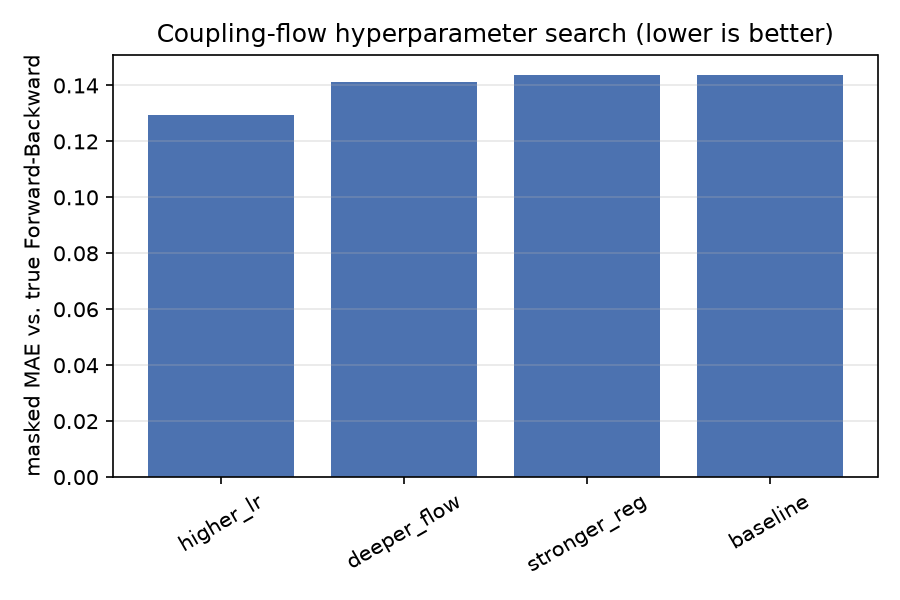
\includegraphics[width=0.48\linewidth]{figures/hyperparameter_search_joint.png}
\caption{Joint pipeline. Left: the coupling flow's training/validation
loss (there is no separate Stage-1 pretraining curve in this design).
Right: masked MAE per configuration in the trimmed 4-configuration search
(lower is better); the higher-learning-rate, depth-$6$ configuration was
selected.}
\label{fig:training_joint}
\end{figure}


\section{Diagnostics}

\subsection{Simulation-Based Calibration (SBC)}

Standard SBC \parencite{sbc} draws parameters from the prior, simulates data, and checks
whether posterior ranks are uniformly distributed. Our setting differs: the HMM parameters
are fixed (not inferred), and the Forward-Backward target is a deterministic function of
the input. We adapt SBC by computing, for each sequence position, the rank of the true
Forward-Backward posterior value within the BayesFlow posterior samples, and testing
uniformity of these ranks.

Figure~\ref{fig:sbc} shows the SBC rank histogram and Probability Integral Transform (PIT)
ECDF. The rank distribution is shifted rightward (mean~0.65, only 27\% of ranks below 0.5),
indicating that the BayesFlow posterior \textbf{systematically underestimates} $P(\alpha)$
relative to the Forward-Backward ground truth. This directional bias, together with the
deviation from uniformity quantified by the Kolmogorov-Smirnov statistic, is consistent
with the deterministic-target nature of this problem and the CouplingFlow's difficulty
modeling exact-zero point masses at position~0 of every sequence.

\begin{figure}
    \centering
    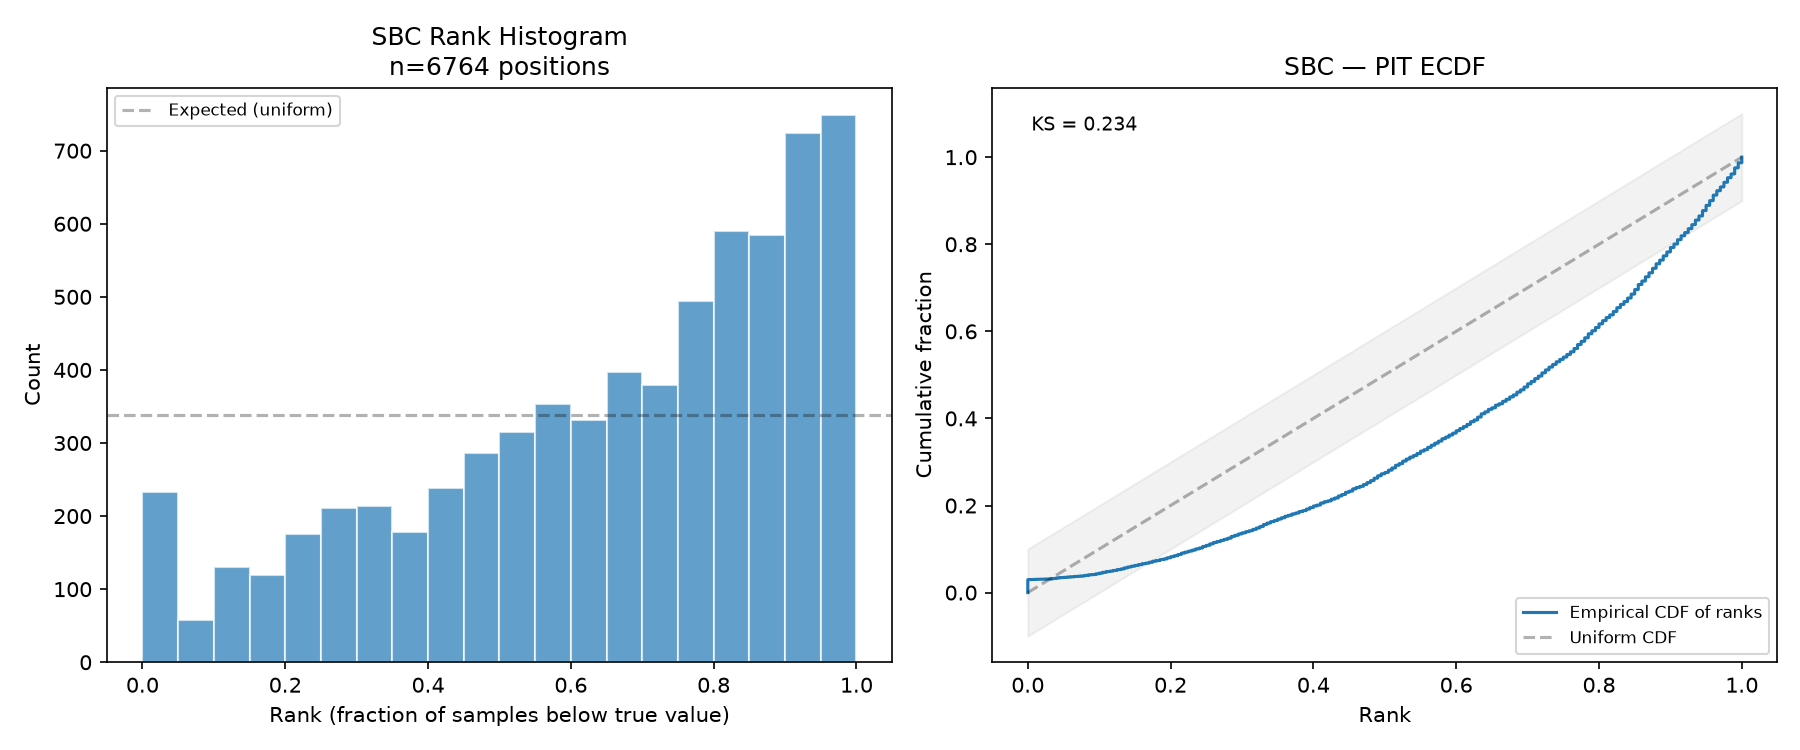
\includegraphics[width=0.95\textwidth]{figures/sbc.png}
    \caption{Adapted SBC diagnostics. Left: rank histogram (uniform if calibrated).
    Right: PIT ECDF with KS statistic.}
    \label{fig:sbc}
\end{figure}

\subsection{Z-score analysis and credible interval coverage}

Per-position z-scores are computed as $z_t = (P_t^{\text{true}} - \hat{\mu}_t) /
\hat{\sigma}_t$, where $\hat{\mu}_t$ and $\hat{\sigma}_t$ are the posterior mean and
standard deviation from BayesFlow samples. For a well-calibrated posterior, z-scores
should approximately follow $\mathcal{N}(0,1)$.

Figure~\ref{fig:zscore} shows the z-score distribution diagnostic. After trimming extreme
outliers (1.1\% of positions retain $|z|<10$), z-scores have mean~0.63 and std~1.27,
indicating a \textbf{systematic positive bias}: the posterior mean underestimates the true
$P(\alpha)$. The credible interval coverage panel (bottom right) shows empirical coverage
\textbf{slightly below} the nominal level at all tested intervals (e.g., 87.3\% vs.\ 90\%
nominal), indicating mild undercoverage rather than conservatism. The combination of
overdispersed z-scores with undercoverage reflects posterior distributions that are
simultaneously too wide in spread but biased in location, so their credible intervals
miss the true value more often than the nominal rate.

\begin{figure}
    \centering
    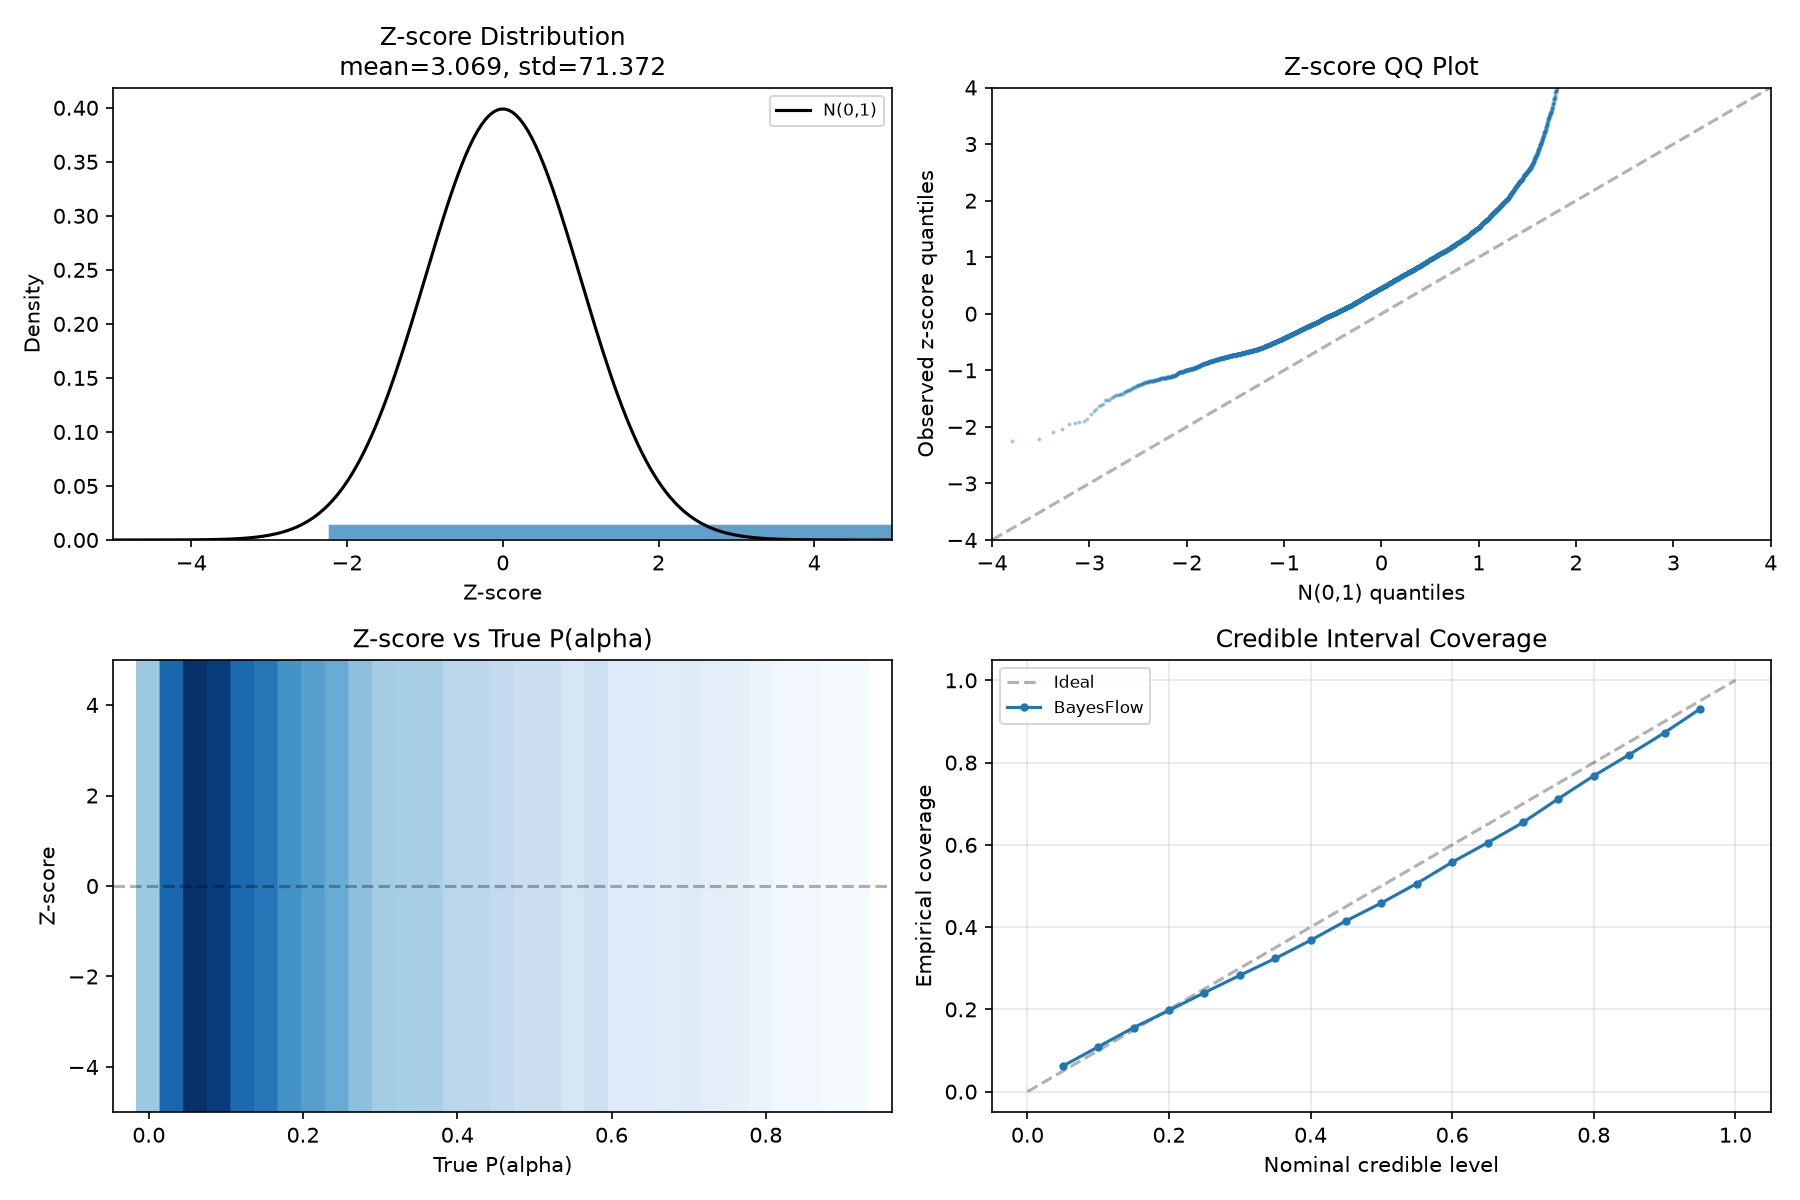
\includegraphics[width=0.95\textwidth]{figures/zscore_coverage.png}
    \caption{Z-score diagnostics. Top left: histogram vs.\ $\mathcal{N}(0,1)$.
    Top right: QQ-plot. Bottom left: z-score vs.\ true $P(\alpha)$.
    Bottom right: empirical vs.\ nominal credible interval coverage.}
    \label{fig:zscore}
\end{figure}

\subsection{Posterior contraction}

Figure~\ref{fig:contraction} illustrates how the BayesFlow posterior contracts around
the true Forward-Backward values on four example sequences. The 90\% credible interval
(shaded blue) typically envelops the true values (black), while the BiLSTM point estimate
(red) tracks them almost perfectly. The BiLSTM's superior accuracy is expected: it is
trained directly on the same BCE objective that defines the target, whereas the
CouplingFlow must model a full conditional density.

\begin{figure}
    \centering
    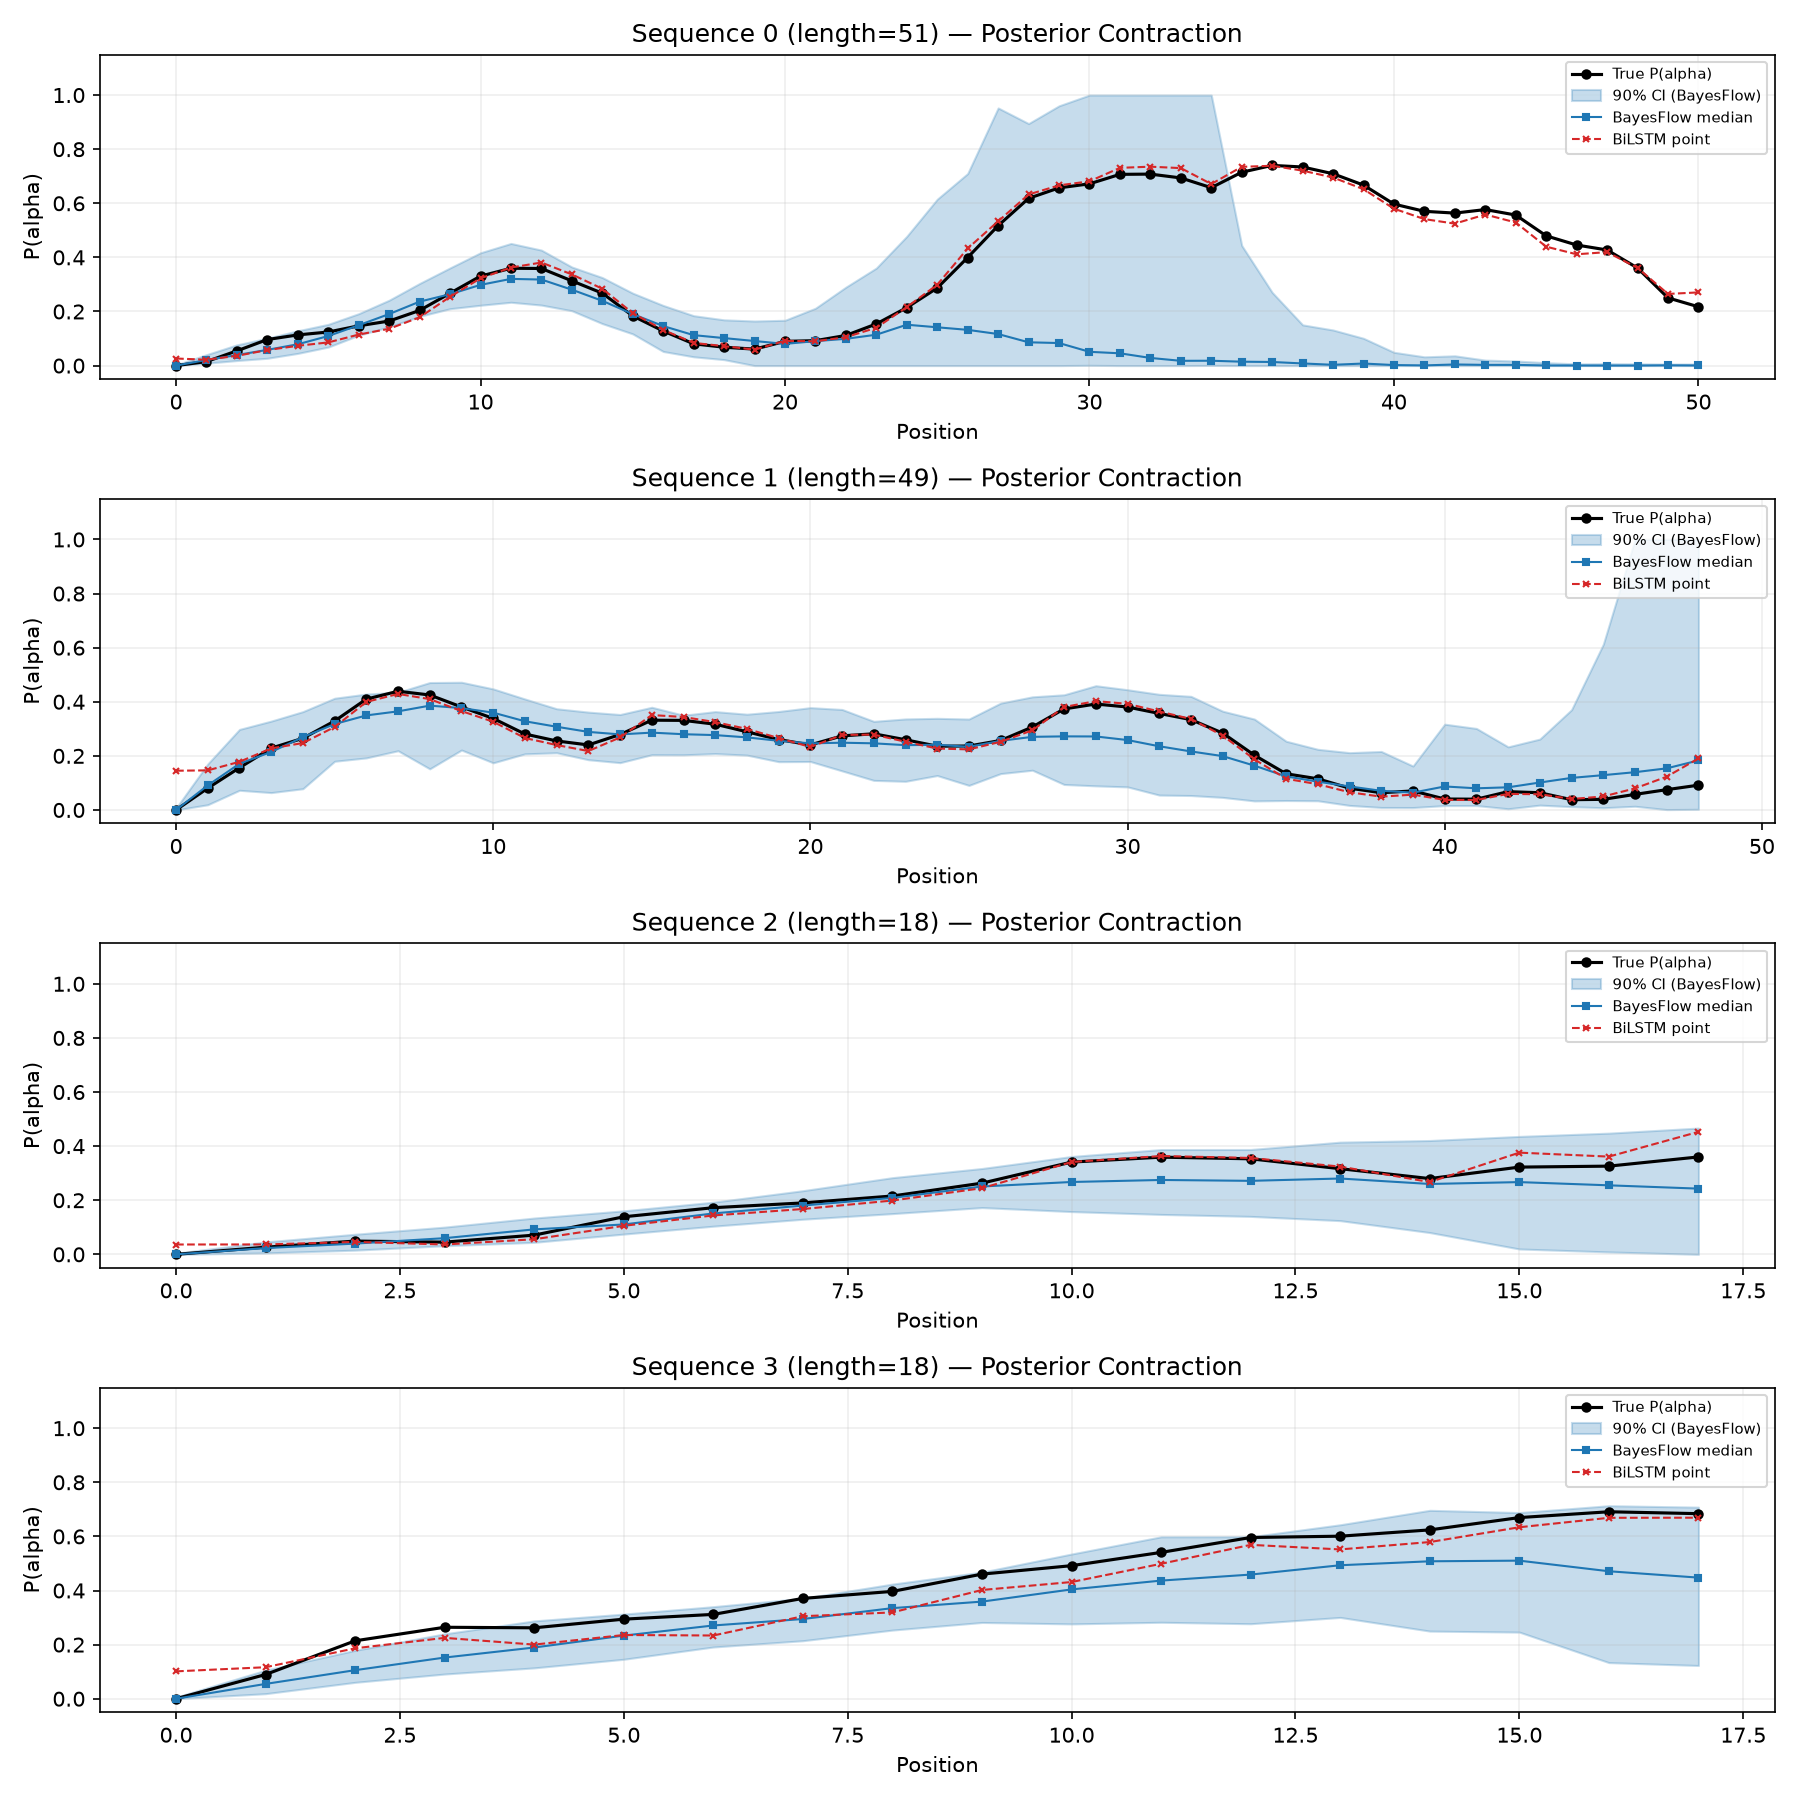
\includegraphics[width=0.95\textwidth]{figures/contraction.png}
    \caption{Per-sequence posterior contraction. Black: true $P(\alpha)$. Blue band:
    BayesFlow 90\% credible interval. Blue squares: BayesFlow median. Red crosses:
    BiLSTM point estimate.}
    \label{fig:contraction}
\end{figure}


\section{Inference}

\subsection{Synthetic held-out evaluation}

Table~\ref{tab:synthetic} reports performance on 200 held-out simulated sequences
(6,764 total residue positions). We compare the BayesFlow point estimate (posterior
median) against the BiLSTM's direct sigmoid output, using the exact Forward-Backward
posterior as ground truth.

\begin{table}
    \centering
    \caption{Performance on held-out simulated data.}
    \label{tab:synthetic}
    \begin{tabular}{l|c|c}
        \hline
        Metric & BayesFlow & BiLSTM \\
        \hline
        MAE & 0.115 & \textbf{0.021} \\
        Pearson correlation & 0.560 & \textbf{0.988} \\
        \hline
    \end{tabular}
\end{table}

The BiLSTM near-perfectly recovers the Forward-Backward posteriors ($r=0.99$), confirming
that a direct neural network can learn the deterministic input–output mapping of the HMM
with high fidelity. The BayesFlow posterior median achieves lower but reasonable accuracy
($r=0.56$), consistent with its role as a density estimator rather than a point predictor.

\subsection{Insulin 1A7F validation}

We evaluate both models on human insulin by comparing predicted $P(\alpha)$ to the
experimental HELIX annotation. Table~\ref{tab:insulin} summarizes per-chain results;
Figure~\ref{fig:insulin} shows the per-residue predictions.

\begin{table}
    \centering
    \caption{Insulin 1A7F validation results.}
    \label{tab:insulin}
    \begin{tabular}{l|c|c|c|c}
        \hline
        Chain & True helix \% & BayesFlow corr & BiLSTM corr & BayesFlow acc. \\
        \hline
        A (21 aa) & 61.9\% & 0.170 & 0.240 & 0.381 \\
        B (29 aa) & 34.5\% & \textbf{0.856} & 0.836 & 0.655 \\
        \hline
    \end{tabular}
\end{table}

\begin{figure}
    \centering
    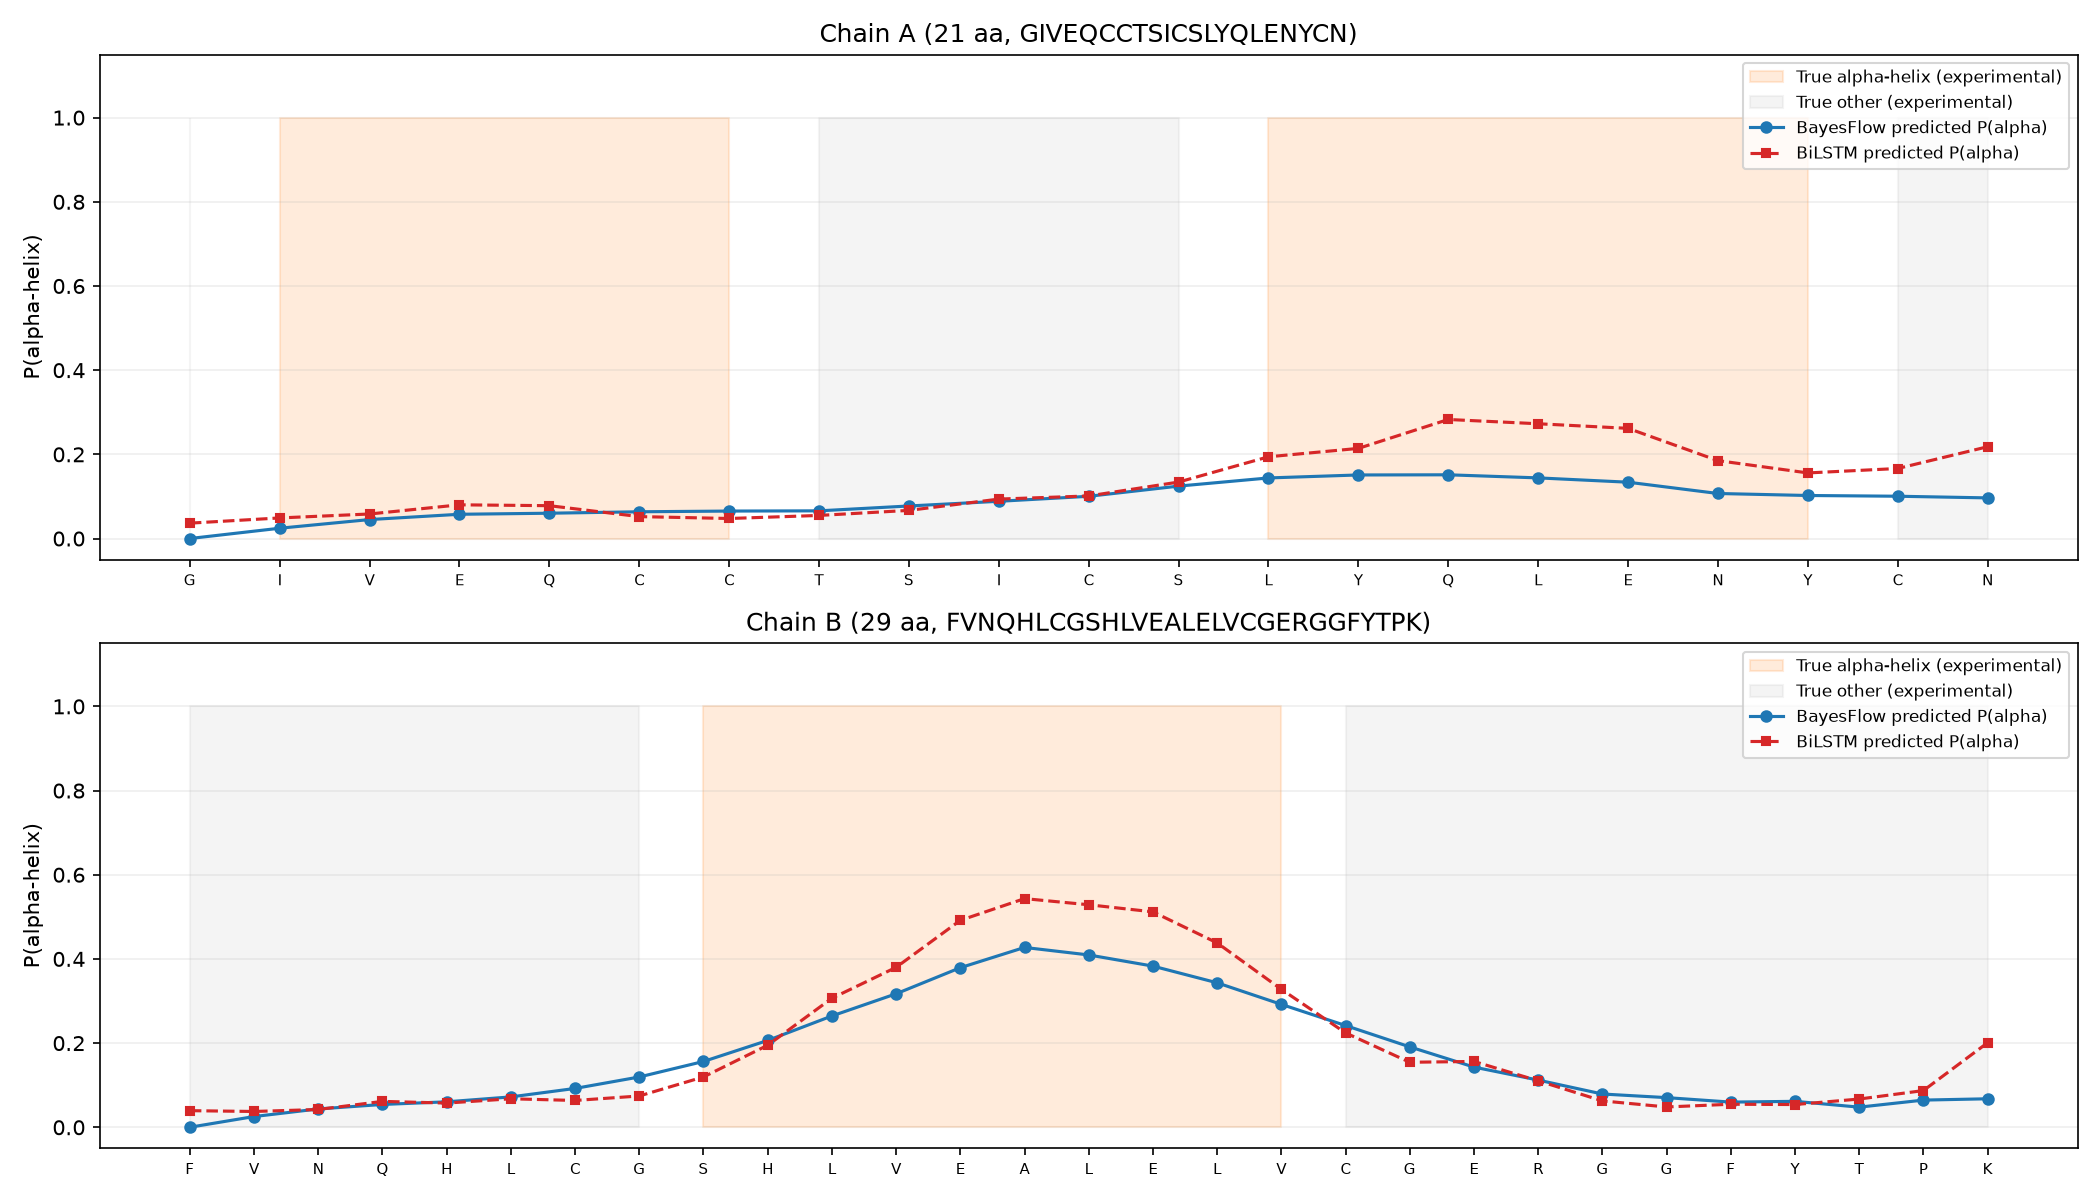
\includegraphics[width=0.95\textwidth]{figures/insulin_predictions.png}
    \caption{Per-residue predicted $P(\alpha\text{-helix})$ for human insulin chains A
    and B (PDB: 1A7F). Orange shading: experimental HELIX annotation. Blue: BayesFlow.
    Red: BiLSTM.}
    \label{fig:insulin}
\end{figure}

Chain B (34.5\% true helix) is predicted well by both models, with BayesFlow achieving
the highest correlation ($r=0.86$). Chain B's helix fraction closely matches the HMM's
stationary distribution ($\pi \approx 33\%$), so the prior does not conflict with the
evidence.

Chain A (61.9\% true helix) is poorly predicted by both models ($r\approx 0.2$). The
HMM's stationary prior of $\sim$33\% helix strongly biases predictions toward
\textit{other}, and the emission tables lack sufficient discriminative information to
override this prior over only 21 residues. Running Forward-Backward \textit{directly}
on the insulin sequence yields similarly poor performance on chain~A ($r\approx 0.40$
vs.\ experimental labels), confirming that this is a limitation of the two-state HMM
model itself, not of the neural approximator.


\section{Discussion \& Conclusion}

\subsection{What BayesFlow contributes}

The BiLSTM point-prediction network outperforms the BayesFlow posterior on raw accuracy
($r=0.99$ vs.\ $0.56$ on synthetic data). This is expected: the Forward-Backward target
is a deterministic function of the input under fixed HMM parameters, so there is no
genuine parameter uncertainty for a density estimator to recover. A direct network can
learn this map more efficiently than a normalizing flow.

However, BayesFlow provides capabilities that a point predictor cannot:
\begin{itemize}
    \item Posterior samples with credible intervals (Figure~\ref{fig:contraction}),
    enabling uncertainty quantification at each residue.
    \item Calibration diagnostics (SBC, z-scores, coverage plots) that assess
    whether the model's uncertainty estimates are trustworthy.
    \item An amortized inference framework that would directly generalize to settings
    with genuine parameter uncertainty, such as inferring the HMM parameters themselves
    from observed sequences.
\end{itemize}

\subsection{Model limitations}

The two-state HMM with fixed empirical emission tables is an oversimplified model of
protein secondary structure. The stationary $\alpha$-helix prior of $\nicefrac{1}{3}$
systematically biases predictions, and the emission tables are not informative enough
to reliably overcome this prior on short sequences. This is most evident on insulin
chain~A, where the model fails regardless of whether inference is performed exactly
(Forward-Backward) or approximately (BayesFlow/BiLSTM).

\subsection{Conclusion}

We successfully implemented a full simulation-based inference pipeline for protein
secondary structure: HMM simulation, Forward-Backward ground-truth generation, BiLSTM
summary network design, BayesFlow CouplingFlow training, and comprehensive calibration
diagnostics including adapted SBC, z-score analysis, and credible interval coverage.
Validation on both synthetic and real data reveals both the strengths of the neural
approximator (faithful learning of the training target, well-behaved uncertainty on
chain~B) and the fundamental limitations of the two-state HMM as a generative model of
real protein structure.

All code, check scripts, and diagnostic outputs are available in the project repository.

\printbibliography

\end{document}
